% ====================================================================
% DIFFERENTIABLE TRACK
% ====================================================================
\chapter{What differentiable simulation is}
\label{ch:d1}

\begin{keybox}
\textbf{Key idea.} A classical solver answers \emph{``what happens?''}.
A differentiable solver also answers \emph{``what should I change?''} ---
it returns the gradient of any scalar output $J$ with respect to any
input parameter $p$ (material coefficients, a process schedule,
geometry). That single object $dJ/dp$ turns the simulator from a
\emph{predictor} into an \emph{instrument for design and inference}. And
because a gradient you cannot trust is worse than none, DiffSim computes
it \emph{three independent ways} and checks that they agree.
\end{keybox}

\section{Why a gradient}

Every question we ask of a morphology simulator downstream --- fit this
material parameter to a measured morphology, choose a quench schedule
that hits a target crystallinity, learn a free-energy functional from
snapshots --- is an \emph{optimization}. Optimization needs a gradient:
$dJ/dp$ says how a scalar objective $J$ (a domain size, an interfacial
area, a crystalline fraction) moves when you nudge a parameter $p$.

The naive way to get $dJ/dp$ is finite differences: run the simulation
at $p+\epsilon$ and $p-\epsilon$ and subtract. That costs \emph{two
forward solves per parameter} and forces you to tune $\epsilon$ (too big:
truncation error; too small: roundoff). With hundreds of parameters --- a
temperature schedule sampled every step, a free energy with many
coefficients --- it is hopeless. The \textbf{adjoint method} returns
$dJ/dp$ for \emph{all} parameters at once, at the cost of a single extra
(linear) solve backward through the trajectory, exact to machine
precision. That $O(1)$-in-parameters cost is what makes design possible.

\section{The three ways to a gradient}

DiffSim's differentiable core (\file{src/diffsim/adjoint/}) computes the
same gradient three ways, and the tutorial runs all three live:

\begin{enumerate}[nosep]
  \item \textbf{Adjoint} --- a hand-derived reverse sweep. We do
        \emph{not} tape the Newton iterations; we differentiate only the
        converged discrete relation $R_n(x_n; x_{\text{hist}}, p)=0$ (the
        implicit-function theorem). For $J=\sum_n j(x_n)$,
        %
        \begin{equation}
          J_n^{\!\top}\lambda_n = \dd{j}{x_n}
            - \!\sum_{k\ge1}\Big(\dd{R_{n+k}}{x_n}\Big)^{\!\top}\!\lambda_{n+k},
          \qquad
          \dd{J}{p} = -\sum_n \lambda_n^{\!\top}\,\dd{R_n}{p},
          \label{eq:d1adj}
        \end{equation}
        %
        where $J_n=\partial R_n/\partial x_n$ is \emph{exactly} the
        Jacobian the forward Newton already assembled at convergence, and
        $\partial R_n/\partial p$ is analytic. This is the production
        capability.
  \item \textbf{Autograd twin} --- a faithful PyTorch reimplementation of
        the \emph{same} discrete solver, differentiated by
        \code{torch.autograd} through the converged Newton loop. Different
        code, a different differentiation engine, the same math: an
        \emph{independent} reference.
  \item \textbf{Finite differences} --- central differences
        $\big(J(p+\epsilon)-J(p-\epsilon)\big)/2\epsilon$. No calculus at
        all; the ground truth every gradient must match, down to the FD
        error floor.
\end{enumerate}

\begin{keybox}
\textbf{The adjoint differentiates the \emph{real} brick.} The discrete
forward in \file{adjoint/phasefield.py} is a vectorised re-implementation
of the production Cahn--Hilliard residual and Jacobian that is
\emph{bit-parity} with \code{CahnHilliardStepper} (measured
$\max|\Delta c|\sim10^{-16}$). So the gradient is taken through the same
operator the research code marches --- not a look-alike toy.
\end{keybox}

\section{Run it}

\begin{runbox}
\textbf{Run it.}
\begin{lstlisting}
cd differentiable/01_three_way_gradient
python run.py            # 9x9 nodes, 3 steps, three-way check
\end{lstlisting}
It marches a short Flory--Huggins Cahn--Hilliard rollout, forms the
scalar objective $J=\tfrac12\lVert c_N-\tfrac12\rVert^2$, and computes
$dJ/d\{M,\kappa,\chi,A\}$ all three ways. It prints the table and
\textbf{self-checks} that the methods agree --- that agreement is the
gate. Compare with \file{EXPECTED.md}.
\end{runbox}

\begin{keybox}
\textbf{Measured self-check} (three-way gradient of
$J=\tfrac12\lVert c_N-\tfrac12\rVert^2$ through a \DoneSteps-step march,
$\DoneSide\times\DoneSide$ nodes).
\begin{center}\small
\begin{tabular}{lc}
\toprule
parameter & adjoint $dJ/dp$ \\
\midrule
$M$ (mobility)      & \DoneGradM     \\
$\kappa$ (gradient) & \DoneGradKappa \\
$\chi=B$ (Flory)    & \DoneGradChi   \\
$A$ (entropic)      & \DoneGradA     \\
\bottomrule
\end{tabular}
\end{center}
Adjoint and autograd twin agree to $\sim$machine precision (worst
$\le\DoneAgreeTwin$): the \emph{same} discrete math, two independent
differentiation engines. Adjoint and finite differences agree to worst
$\le\DoneAgreeFD$: the FD truncation/roundoff floor.
\end{keybox}

% --- generated by gen_figures.py ---
\begin{figure}[h]\centering
  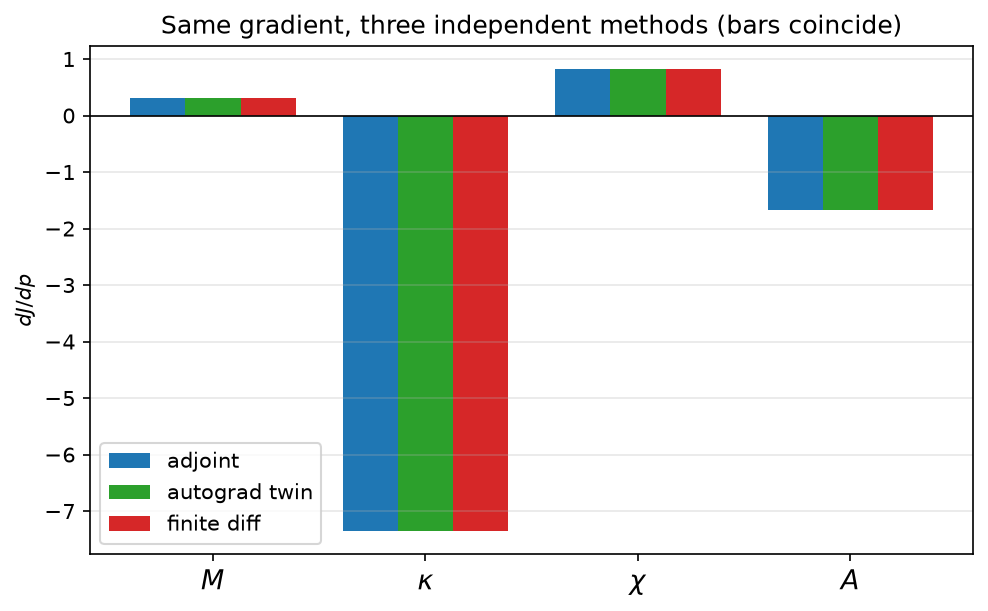
\includegraphics[width=0.86\linewidth]{figures/d1_agreement.png}
  \caption{The same gradient, three ways. For each parameter the adjoint,
    autograd-twin, and finite-difference bars are \emph{visually
    coincident} --- that overlap is the message: three independent methods
    return one number. The signs are physical (raising $\chi$ drives the
    field away from the uniform $c=\tfrac12$, so $J$ grows;
    $dJ/d\chi>0$).}
  \label{fig:d1agree}
\end{figure}

\begin{figure}[h]\centering
  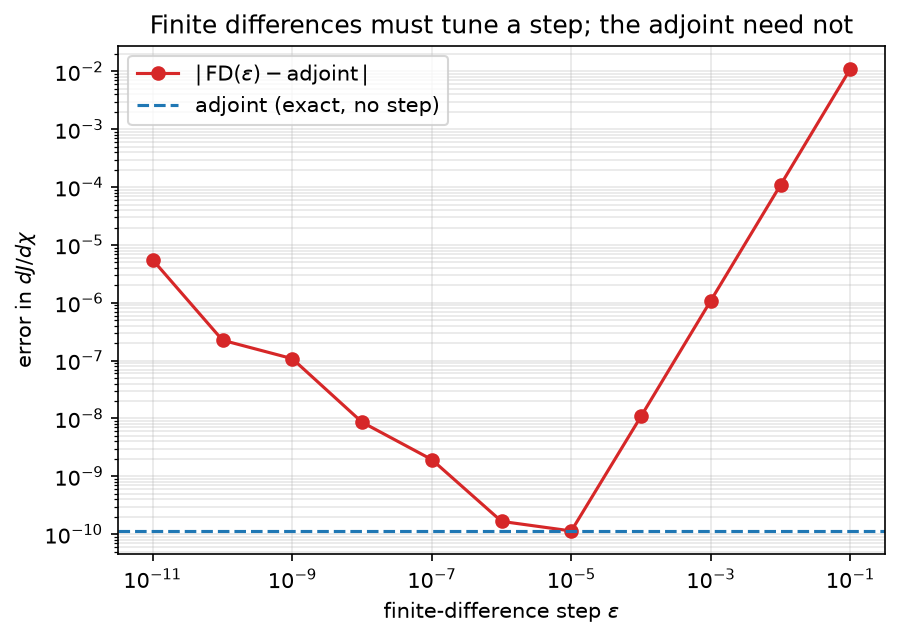
\includegraphics[width=0.66\linewidth]{figures/d1_fd_valley.png}
  \caption{Why the adjoint, not finite differences. The error of the
    central difference for $dJ/d\chi$ is a V-shaped function of the step
    $\epsilon$: on the right, $O(\epsilon^2)$ truncation error falls as
    $\epsilon$ shrinks; on the left, catastrophic cancellation (roundoff)
    takes over and it rises. The valley floor (best FD $\approx
    \DoneFDfloor$) is the most FD can achieve --- and it sits far above the
    adjoint, which is exact and needs no step to tune.}
  \label{fig:d1valley}
\end{figure}

\section{Code walk-through}

The tutorial's core is \file{three\_way.py}; it drives
\file{src/diffsim/adjoint/phasefield.py}.

\paragraph{1. One reverse sweep, all gradients.}
\begin{lstlisting}
fwd = CHForward(dm, FHEnergy(A, B), M=M, kappa=kappa, dt=dt, order=order)
fwd.set_initial(ic); fwd.run(n_steps)               # record the trajectory
dJdx = [zeros] * n_steps
dJdx[-1][0::2] = fwd.steps[-1]["c"] - target         # dj/dc on the final step
g_adj = CHAdjoint(fwd).gradient(dJdx, ["M","kappa","B","A"])
\end{lstlisting}
\code{gradient} runs \eqref{eq:d1adj} backward through the recorded
steps and returns \emph{every} $dJ/dp$ from that one sweep.

\paragraph{2. The independent twin.}
\begin{lstlisting}
twin = CHTwin(dm, energy="fh", dt=dt, order=order, device="cpu")
out  = twin.march(c0, None, M, kappa, dict(A=A, B=B), n_steps)  # leaf tensors
loss = 0.5 * ((out[-1][0] - target)**2).sum();  loss.backward()
\end{lstlisting}
Autograd differentiates through the converged Newton iterations; because
the loop is driven to a tight residual, that returns the same
implicit-function-theorem gradient the hand adjoint derives.

\paragraph{3. The ground truth.}
Central differences on each parameter --- two forward solves apiece --- with
no calculus, is what pins the other two to reality.

\section{Explore on your own}

\question{Switch to BDF2 (\code{--order 2 --steps 4}). The
variable-coefficient history now couples \emph{two} previous steps into
each residual; does the three-way agreement survive? (It must --- the
adjoint's history cotangent carries both slots.)}

\question{Add a second objective, e.g.\ the interfacial energy
$\tfrac{\kappa}{2}\lVert\grad c_N\rVert^2$. Re-derive its seed
$dj/dc_N$ and confirm the adjoint still matches finite differences.}

\question{Time the adjoint vs.\ finite differences as you add parameters
(say, a per-step schedule of length $N$). The adjoint cost is flat in
$N$; the FD cost grows linearly. At what $N$ does the crossover make FD
impractical?}

\question{Shrink the FD step $\epsilon$ toward $10^{-12}$ and watch the
error in Fig.~\ref{fig:d1valley} \emph{rise}. Explain why, and why the
adjoint has no analogous floor.}

% ====================================================================
\chapter{Morphology sensitivity}
\label{ch:d2}

\begin{keybox}
\textbf{Key idea.} With the gradient now trustworthy, ask a physical
question: how sensitive is the \emph{morphology} to the material
parameters? Pick a scalar summary of the pattern --- here the
\emph{demixing amplitude} $J=\tfrac12\lVert c_N-\bar c\rVert^2$, the
spatial variance of the composition --- and the adjoint returns
$dJ/d\chi$ and $dJ/d\kappa$ in one sweep. The \emph{signs} are the
physics: $dJ/d\chi>0$ (interaction sharpens the pattern),
$dJ/d\kappa<0$ (gradient penalty blurs it).
\end{keybox}

\section{A scalar handle on the morphology}

A morphology is a whole field; to differentiate we need a scalar. Any
morphology metric will do --- domain size, interfacial area, a structure
factor --- and the adjoint machinery is identical: pick $J(c_N)$, hand it
the seed $dj/dc_N$, get every $dJ/dp$. We use the demixing amplitude
%
\begin{equation}
  J(c_N) = \tfrac12\sum_i\big(c_{N,i}-\bar c\big)^2 ,
  \qquad \bar c=\text{mean}(c_0),
  \label{eq:d2J}
\end{equation}
%
which is small for a nearly uniform blend and grows as the two phases
separate --- a scalar proxy for ``how demixed is the film''. Because the
Cahn--Hilliard dynamics conserve mass, $\bar c$ is fixed by the initial
condition, so the seed
$dj/dc_N = (c_N-\bar c)$ is exact and clean.

The two sensitivities have opposite, and physical, signs. Above the
spinodal ($\chi>2A$) a larger interaction $\chi$ deepens the enthalpic
well and drives demixing harder, so $J$ grows: $dJ/d\chi>0$. The
gradient penalty $\tfrac{\kappa}{2}|\grad c|^2$ instead \emph{opposes}
composition variation --- a larger $\kappa$ thickens interfaces and
smooths the field --- so $dJ/d\kappa<0$. The adjoint recovers both, and
finite differences confirm them.

\section{Run it}

\begin{runbox}
\textbf{Run it.}
\begin{lstlisting}
cd differentiable/02_morphology_sensitivity
python run.py            # dJ/dchi and dJ/dkappa, FD-verified
\end{lstlisting}
It marches a short Flory--Huggins rollout at $\chi=\DtwoChi$,
$\kappa=\DtwoKappa$ (interior data, so the logs stay smooth), forms
\eqref{eq:d2J}, and prints $dJ/d\chi$, $dJ/d\kappa$ with their
finite-difference checks and sign assertions. Compare with
\file{EXPECTED.md}.
\end{runbox}

\begin{keybox}
\textbf{Measured self-check} (\DtwoSteps-step march, $\chi=\DtwoChi$,
$\kappa=\DtwoKappa$).
\begin{center}\small
\begin{tabular}{lcc}
\toprule
 & value & meaning \\
\midrule
demixing amplitude $J$ & \DtwoJ & how separated the blend is \\
$dJ/d\chi$   & \DtwoGradChi   & $>0$: interaction sharpens \\
$dJ/d\kappa$ & \DtwoGradKappa & $<0$: gradient penalty blurs \\
worst adjoint-vs-FD    & \DtwoRelFD & the FD-verified gate \\
\bottomrule
\end{tabular}
\end{center}
\end{keybox}

% --- generated by gen_figures.py ---
\begin{figure}[h]\centering
  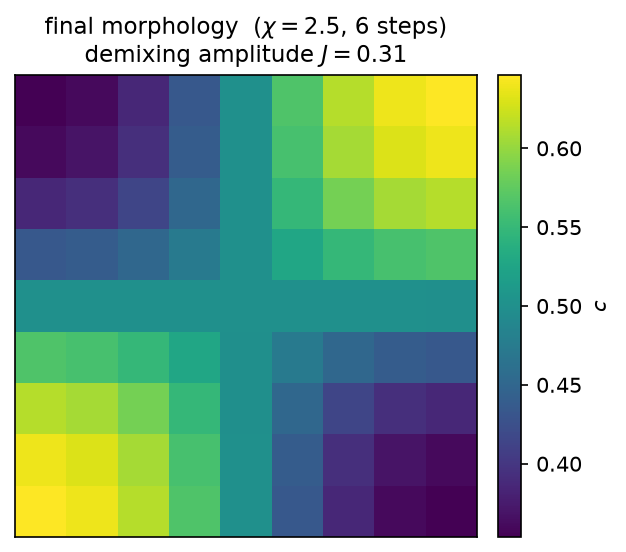
\includegraphics[width=0.46\linewidth]{figures/d2_morphology.png}\hfill
  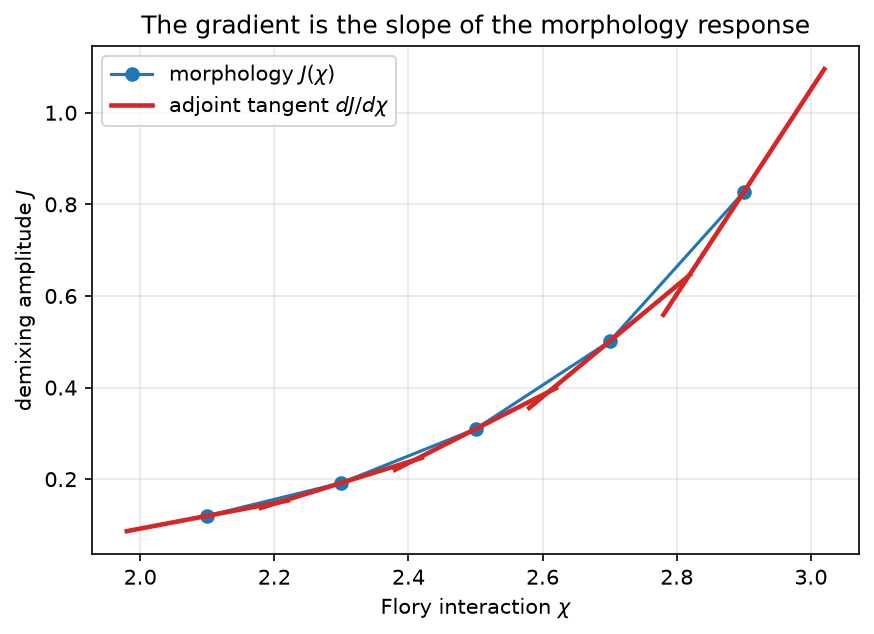
\includegraphics[width=0.52\linewidth]{figures/d2_slope.png}
  \caption{Left: the final morphology whose scalar summary $J$ we
    differentiate. Right: the demixing amplitude $J(\chi)$ sampled across
    interaction strengths (blue), with the adjoint tangents $dJ/d\chi$
    (red) drawn at each point. The tangents lie \emph{along} the response
    curve --- the gradient is the local slope of the morphology's answer
    to a change in $\chi$.}
  \label{fig:d2}
\end{figure}

\section{Code walk-through}

The seed is the only thing that changes from D1; the adjoint sweep is
identical.
\begin{lstlisting}
fwd, cN = march(dm, coords, chi, kappa, n_steps)   # short CH rollout
dJdx[-1][0::2] = cN - c_bar                          # dj/dc_N for eq. (D2)
g = CHAdjoint(fwd).gradient(dJdx, ["B", "kappa"])   # -> dJ/dchi, dJ/dkappa
\end{lstlisting}
Swap in any other differentiable morphology metric --- redefine $J(c_N)$
and its seed --- and the same call returns its sensitivities. That
substitutability is the point: the adjoint does not care what scalar you
put on top of the field.

\section{Explore on your own}

\question{Replace the demixing amplitude with a genuine interfacial-area
proxy, $J=\tfrac12\lVert\grad c_N\rVert^2$. Derive its seed and check the
sign of $dJ/d\kappa$ --- does a thicker interface raise or lower this
metric?}

\question{Sweep $\chi$ from below the spinodal ($\chi<2$) to well above.
Where does $dJ/d\chi$ turn on, and does the onset line up with the
spinodal threshold from Physics~P1?}

\question{Push the rollout longer (\code{--steps 20}) and watch the
Flory--Huggins logs approach the walls. At what point does the forward
solve fail, and what does that tell you about differentiating stiff free
energies near the pure phases?}
\chapter{Recovering parameters from a morphology}
\label{ch:d3}
\emph{Under construction --- fit $\chi,\kappa$ to a target morphology by
gradient descent.}
\chapter{Process gradients}
\label{ch:d4}
\emph{Under construction --- gradient with respect to the quench
schedule $T(t)$, as a time series.}
\chapter{Crystallinity sensitivity}
\label{ch:d5}
\emph{Under construction --- differentiating a crystallinity metric
through the coupled $\phi,\psi$ crystallization fields.}
\chapter{Learning the free energy from snapshots}
\label{ch:d6}
\emph{Under construction --- recover a parametrized $f(c)$ from a time
series of morphology snapshots.}
\chapter{Capstone: inverse-designing a process}
\label{ch:d7}
\emph{Under construction --- optimize a $T(t)$ schedule to hit a target
crystalline fraction.}
